\documentclass[11pt]{article}
\usepackage{../stat110}
\usepackage{graphicx}
\usepackage{epigraph}

%\STAFF

\begin{document}
\SectionNotes{2}{Probability and Story Proofs - Continued}{Luis Perez (luisperez@college.harvard.edu)}{Aidi Zhang (aidizhang@college.harvard.edu)}{2}

\setlength{\epigraphwidth}{.6\textwidth}
\epigraph{The most important questions of life are indeed, for the most part, really only problems of probability.}{Pierre Simon Laplace}

\section*{Administrivia}
Our section handouts will be posted online before 9am on Tuesdays. Solutions will be posted before 12pm on Wednesday, or soon after Aidi's section.

The below review notes are courtesy of William Chen and Sebastian Chiu, with small modifications.
\section*{Story Proofs}
\begin{description}
  \item[Definition] - A proof by interpretation or application rather than by algebra or calculus. Examples of story proofs would be combinatorial proofs, which there are three examples of below, where two quantities are equated as it it shown that they are two ways of counting the same thing.
  \item[Example 1] - Symmetry Rule for Binomial Coefficients
    \[{n \choose k} = {n \choose n-k}\]
    If you want to choose $k$ people out of $n$, you can either directly pick the $k$ people to be included (LHS), or pick the $n-k$ to be not included (RHS).
  \item[Example 2] - Product of ${r \choose m}$ with ${m \choose k}$
    \[{r \choose m}{m \choose k} = {r \choose k}{r-k \choose m-k}\]
    In a class of $r$, you want to pick a team of $m$ members with $k$ leaders. You can either first choose the team (${r \choose m}$ ways) and then the leaders out of the team (${m \choose k}$ ways) (LHS), or you first choose the leaders (${r \choose k}$ ways) and then choose the remaining members out of the remainder of the class (${r-k \choose m-k}$ ways) (RHS).
  \item[Example 3] - Vandermonde Identity
    \[\sum_{i=0}^k {m \choose i}{n \choose k-i} = {m + n \choose k}\]
    A class contains $m$ females and $n$ males. We want to find all of the ways to form teams of $k$ students. We can find the number of teams that include $i$ females - there are ${m \choose i}$ ways to choose the females and ${n \choose k-i}$ ways to choose the males, for a total of ${m \choose i}{n \choose k-i}$ ways to choose a team with $i$ females. We sum over $i$ to get the total number of teams (LHS), which we know is also ${m + n \choose k}$ (RHS).
\end{description}

\section*{Set Theory and Statistics}
%To understand probability it helps to understand basic set theory. An \emph{event} is a set in that it is a collection of possible outcomes of an experiment (or a subset of the sample space). With set theory we can talk about things like unions, intersections, or complements of events.

\begin{description}
  \item[Sets and Subsets] - A set is a collection of distinct objects. $A$ is a subset of $B$ if every element of $A$ is also included in $B$. %If a subset contains the elements 1, 2, 3, the the set that includes those elements is denoted $\{1, 2, 3\}$
  \item[Set Notation] - Note that ${\bf {\bf A}} \cup {\bf B}$, ${\bf A} \cap {\bf B}$, and ${\bf A^c}$ are all sets too.
  \begin{description}
    \item[Union] - ${\bf A} \cup {\bf B}$ (read \emph{{\bf A} union {\bf B}}) means ${\bf A}\ or\ {\bf B}$
    \item[Intersection] - ${\bf A} \cap {\bf B}$ (read \emph{{\bf A} intersect {\bf B}}) means ${\bf A}\ and \ {\bf B}$
    \item[Complement] - ${\bf A^c}$ (read \emph{{\bf A} complement}) occurs whenever ${\bf A}$ does not occur
  \end{description}
  \item[Disjoint Sets] - Two sets are disjoint if their intersection is the empty set (e.g. they don't overlap).
  \item[Empty Set] - The empty set, denoted $\emptyset$, is the set that contains nothing.
  \item[Partition] - A set of subsets ${\bf A}_1, {\bf A}_2, {\bf A}_3, ... {\bf A}_n$ partition a space if they are disjoint (mutually exclusive) and exhaustive (e.g. they cover all possible outcomes, or their union is the entire set). A simple case of a partitioning set of subsets is ${\bf A}, {\bf A^c}$
  \item[Experiments/Outcomes] - An experiment generates an outcome from a pre-determined list. For example, a dice roll generates outcomes in the set $\{1, 2, 3, 4, 5, 6\}$
  \item[Sample Space] - The sample space, denoted $\Omega$, is the set of possible outcomes. Note that the probability of this event is 1, since something in the sample space will always occur.
  \item[Event] - An event is a subset of the sample space, or a collection of possible outcomes of an experiment. We say that the event has occurred if any of the outcomes in the event have happened.
\end{description}

\section*{Disjointness Versus Independence}

  \begin{description}
    \item[Disjoint Events] - ${\bf A}$ and ${\bf B}$ are disjoint when they cannot happen simultaneously, or
      \begin{align*}
      P({\bf A} \cap {\bf B}) &= 0\\
      {\bf A} \cap {\bf B} &= \emptyset
      \end{align*}
    \item[Independent Events] - ${\bf A}$ and ${\bf B}$ are independent if knowing one gives you no information about the other. ${\bf A}$ and ${\bf B}$ are independent if and only if one of the following equivalent statements hold:
       \begin{align*}
      P({\bf A}\cap {\bf B}) &= P({\bf A})P({\bf B}) \\
      P({\bf A}|{\bf B}) &= P({\bf A})
       \end{align*}

    \item[Conditional Independence] - ${\bf A}$ and ${\bf B}$ are conditionally independent given ${\bf C}$ if: $P({\bf A}\cap {\bf B}|{\bf C}) = P({\bf A}|{\bf C})P({\bf B}|{\bf C})$. Conditional independence does not imply independence, and independence does not imply conditional independence.
  \end{description}

\section*{Unions, Intersections, and Complements}

  \begin{description}

    \item[De Morgan's Laws] - Gives a useful relation that can make calculating probabilities of unions easier by relating them to intersections, and vice versa. De Morgan's Law says that the complement is distributive as long as you flip the sign in the middle.
       \begin{align*}
    ({\bf A} \cup {\bf B})^c \equiv {\bf A^c} \cap {\bf B^c} \\
    ({\bf A} \cap {\bf B})^c \equiv {\bf A^c} \cup {\bf B^c}
       \end{align*}

    \item[Complements] - The following are true.
       \begin{align*}
       {\bf A} \cup {\bf A}^c &= \Omega \\
       {\bf A} \cap {\bf A}^c &= \emptyset\\
       P({\bf A}) &= 1 -  P({\bf A}^c)
       \end{align*}

    \item[Principle of Inclusion-Exclusion] - Helps you find the probabilities of unions of events.
    \[ P ({\bf A} \cup {\bf B}) = P({\bf A}) + P({\bf B}) - P({\bf A} \cap {\bf B}) \]
    \[ P ({\bf A} \cup {\bf B} \cup {\bf C}) = P({\bf A}) + P({\bf B}) + P({\bf C}) - P({\bf A} \cap {\bf B}) - P({\bf B} \cap {\bf C}) - P({\bf A} \cap {\bf C}) + P({\bf A} \cap {\bf B} \cap {\bf C})\]
    \[P(\textnormal{Union of many events}) = \textnormal{Singles} - \textnormal{Doubles} + \textnormal{Triples} - \textnormal{Quadruples} \dots \] \\
Sometimes you can avoid Inclusion-Exclusion by using the complement. The probability that at least one of $A_i$ happen is equal to 1 minus the probability that none of them happen.
    \begin{align*}
      P(A_1 \cup A_2 \cup \dots \cup A_n) &= 1 - P((A_1 \cup A_2 \cup \dots \cup A_n)^c) \\
      &= 1 - P(A_1^c \cap \dots \cap A_n^c)
    \end{align*}

  \end{description}

\section*{Joint, Marginal, and Conditional Probabilities and Bayes' Rule}

  \begin{description}
    \item[Joint Probability] - $P({\bf A} \cap {\bf B}) $ or $P({\bf A}, {\bf B})$ - Probability of ${\bf A}$ \emph{and} ${\bf B}$.
    \item[Marginal (Unconditional) Probability] - $P({\bf A})$ - Probability of ${\bf A}$
    \item[Conditional Probability] - $P({\bf A}|{\bf B})$ - Probability of ${\bf A}$ given ${\bf B}$ occurred.
    \item[Conditional Probability is Probability] - $P({\bf A}|{\bf B})$ is a probability as well, restricting the sample space to ${\bf B}$ instead of $\Omega$. Any theorem that holds for probability also holds for conditional probability.
    \item[Bayes' Rule] - Bayes' Rule unites marginal, joint, and conditional probabilities. This is \emph{the most important concept of the week}, and one of the backbones of statistics. We use this as the definition of conditional probability.
  \[\boxed{P({\bf A}|{\bf B}) = \frac{P({\bf A} \cap {\bf B})}{P({\bf B})} = \frac{P({\bf B}|{\bf A})P({\bf A})}{P({\bf B})}}\]

  \end{description}

\section*{Law of Total Probability}

\begin{figure}[h!]\centering
  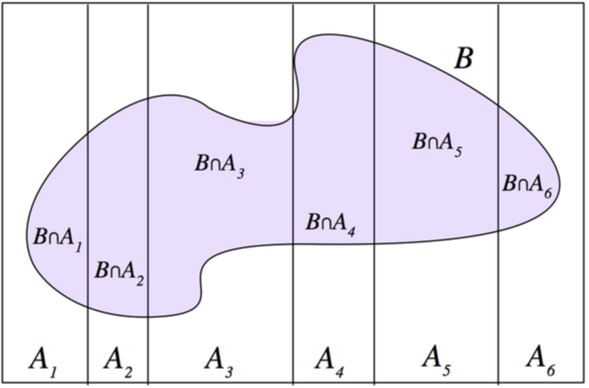
\includegraphics[width = 0.7\textwidth]{LOTP.jpg}
  \caption{The $A_i$ partition the sample space. $P(B)$ is equal to $\sum_i P (B \cap A_i)$. Image from textbook}
\end{figure}

This is a useful way to break up a harder problem into simpler pieces, conditioning on what we wish we knew. For any event B and set of events ${\bf A}_1, {\bf A}_2, {\bf A}_3, ... {\bf A}_n$ that partition a space, the following are true:
   \begin{align*}
P({\bf B}) &= P({\bf B} | {\bf A}_1)P({\bf A}_1) + P({\bf B} | {\bf A}_2)P({\bf A}_2) + ...  P({\bf B} | {\bf A}_n)P({\bf A}_n)\\
P({\bf B}) &= P({\bf B} \cap {\bf A}_1)+ P({\bf B} \cap {\bf A}_2)+ ...  P({\bf B} \cap {\bf A}_n)
   \end{align*}
   or in the simplest case where $A$ is just any event
   \begin{align*}
P({\bf B}) &= P({\bf B} | {\bf A})P({\bf A}) + P({\bf B} | {\bf A^c})P({\bf A^c}) \\
P({\bf B}) &= P({\bf B} \cap {\bf A})+ P({\bf B} \cap {\bf A^c})
   \end{align*}

\section*{A Tale of Two Series}
\begin{minipage}{0.45\textwidth}
\textbf{Geometric Series}
\[\sum_{n=0}^\infty x^n = \frac{1}{1 - x}, |x| < 1\]
\end{minipage}
\hfill
\begin{minipage}{0.45\textwidth}
\textbf{Taylor Series for $e^x$}
\[\sum_{n=0}^\infty \frac{x^n}{n!} = e^x\]
\end{minipage}

These will show up in future problem sets.

\pagebreak

\section*{Practice Problems}
\vskip .2 in

\begin{exercise}
\textbf{The Leaders are Few.} Give a story proof for the following identity:
$$
\sum_{k=1}^{n} k {n \choose k} = n2^{n-1}
$$
\end{exercise}
\begin{solution}
Consider a group of $n$ people, and you're tasked with selecting a non-empty committee and a chair person for that committee. How many ways are there to do this? In the LHS, we could first select a committee of size $k$ for $k \geq 1$, followed by selecting a chair person. The total number of non-empty committees is the sum over all possible sizes.

On the other hand, we could also first select a chair person (with $n$ possibilities). Then we select a subset of the remaining $n-1$ people, of which there are $n-1$. This is given by the LHS.
\end{solution}

\begin{exercise}
\textbf{Democracy to the Rescue!} Give a story proof for the following identity:
$$
\sum_{k=j}^n \sum_{j=0}^n \binom{n}{j} \binom{n-j}{k-j} = 3^n
$$
\end{exercise}
Hint: For these problems, we usually think of selecting a committee. Think about what happens when you select sub-committees.
\begin{solution}
The story is that we have $n$ members of a team, and we need a committee of $k$ people. Out of these $k$ people, we need to choose a very special sub-committee of $j$ people. The constraints on the problem are that $0 \le j \le k \le n$ (having no committee nor special sub-committee is allowed). On the right hand side, we have that every one of the $n$ members can select to be 1. in the sub-committee and hence in the committee, 2. in the committee but not in sub-committee, or 3. not in committee at all. All of them choose independently of each other, hence there are $3^n$ possible permutations.\\
\\
On the left hand side, we first choose a sub-committee of $j$ people out of $n$, and then out of the remaining $n-j$ unassigned members, choose the rest of the $k-j$ people who are in the committee but not sub-committee. The two summations sum this up perfectly.\\
\\
Plug this into Wolfram alpha for sanity checks if you are so inclined! Try to think of other possible story-provable statements. This one Luis and Aidi randomly pulled out of their heads :)
\end{solution}

\begin{exercise}
\textbf{Achieving The Highest Score.} (Taken from Degroot example 2.3.5) Luis rolls a fair 50-sided die with the sides numbered 1 through 50. Let the result of the first roll be $X$. Luis then continues to roll until he obtains another result $Y$ such that $Y \ge X$. Assume all rolls of the die are independent. What is the probability that $Y = 50$?
\end{exercise}
\begin{solution}
Let $A$ be the event that $Y = 50$, and let $B_i$ be the event that the first roll is $i$ for $i = 1,2,3...,50$. We condition on the outcome of the first roll and apply Law of Total Probability (LOTP):

$$P(A) = P(A|B_1)P(B_1) + ... + P(A|B_{50})P(B_{50}) = \frac{1}{50} (\frac{1}{50} + \frac{1}{49} + ... + \frac{1}{2} + 1) \approx 0.09$$
\end{solution}

\begin{exercise}
\textbf{The Homework Return Fiasco.} Suppose all $n$ students in Stat 110 get their first homework back in random order. (This will hopefully not be the case.) What is the probability that at least one student gets his/her correct homework?
\end{exercise}
\begin{solution}
For the observant, this question is actually isomorphic to de Montmort's problem (found on page 22 of the textbook). Let $A_i$ be the event that ith student gets back the ith hat. We are interested in the probability of union $A_1 \cup A_2 \cup ... \cup A_n$. We use inclusion-exclusion to find the probability of this union. First,

$$P(A_i) = \frac{1}{n}$$

This is because using the naive definition of probability, out of the $n!$ possible orderings of the deck, all equally likely, $(n-1)!$ orderings are favorable to $A_i$. Then, for all $1 \le i,j \le n$,

$$P(A_i \cap A_j) = \frac{(n-2)!}{n!} = \frac{1}{n(n-1)}$$

by similar reasoning. This pattern continues for intersections of more events. Using the inclusion-exclusion formula, there are $n$ terms involving one event, $\binom{n}{2}$ terms involving two events, $\binom{n}{3}$ terms involving three events, etc, hence

$$P(\cup_{i=1}^{n}) = \frac{n}{n} - \frac{\binom{n}{2}}{n(n-1)} + \frac{\binom{n}{3}}{n(n-1)(n-2)} - ... + (-1)^{n+1} \cdot \frac{1}{n!} = 1 - \frac{1}{2!} + \frac{1}{3!} - ... + (-1)^{n+1} \cdot \frac{1}{n!}$$

Using the Taylor's series, we see that for large $n$ (which is a good assumption for the actual number of Stat 110 students this year - yay we are happy to have you!), the final probability is close to $1 - \frac{1}{e}$.

\end{solution}

\begin{exercise}
\textbf{The Three-Cornered Duel.} (Taken from Mosteller, Fifty Challenging Problems in Probability) Luis, Aidi and Prof Blitzstein are to fight a three-cornered pistol duel. All know that Aidi's chance of hitting her target is $0.3$, Luis's is $0.5$, and Prof Blitzstein never misses (this somewhat realistically reflects their respective accuracy rates for solving Stat 110 problems). They are to fire at their choice of target in succession in the order Aidi, Prof Blitzstein and Luis, cyclically (but a hit man loses further turns and is no longer shot at) until only one man is left unhit. What should Aidi's strategy be?
\end{exercise}
\begin{solution}
Aidi sees that if she hits Luis, Prof Blitzstein will surely hit her, so she is not going to shoot at Luis. If she shoots at Prof Blizstein and misses him, then Prof clearly shoots the more dangerous Luis first, and Aidi gets one shot at Prof with probability $0.3$ of succeeding. On the other hand, suppose she shoots and hits Prof. Then Luis and Aidi shoot alternately until one hits. Aidi's chance of winning is

$$0.5 \cdot 0.3 + 0.5^2 \cdot 0.7 \cdot 0.3 + 0.5^3 \cdot 0.7^2 \cdot 0.3 + ...$$

Each term corresponds to a sequence of misses by both Luis and Aidi ending with a final hit by Aidi. Summing the geometric series, we get

$$0.5 \cdot 0.3 \cdot (1 + 0.5 \cdot 0.7 + (0.5 \cdot 0.7)^2 + ...) = \frac{0.5 \cdot 0.3}{1 - 0.5 \cdot 0.7} = \frac{3}{13} < 0.3$$

Thus hitting Prof and finishing off with Luis has less probability of winning for Aidi than just missing the first shot. So Aidi fires her first shot into the ground and then tries to hit B with her next shot. Interesting, eh?

\end{solution}

\begin{exercise}
\textbf{Diseases and Parenthood.} A certain hereditary disease can be passed from a mother to her children. Given that the mother has the disease, her children independently will have it with probability 1/2. Given that she doesn't have the disease, her children won’t have it either. A certain mother, who has probability 1/3 of having the disease, has two children (Courtesy of Viviana).
\begin{enumerate}
\item Find the probability that neither child has the disease?
\item Is whether the elder child has the disease independent of whether the younger child has the
disease?
\item The elder child is found not to have the disease. A week later, the younger child is also found
not to have the disease. Given this information, find the probability that the mother has the disease.
\end{enumerate}
\end{exercise}
\begin{solution}
As always, it's helpful to label events :)
\begin{enumerate}
\item Let $M$ be the event that the mother has the disease, and let $C_i$ be the vent that the $i$ child has the disease, for $i \in \{1,2\}$. Then we need to find $P(C_1^c \cap C_2^c)$.
$$
P(C_1^c \cap C_2^c) = P(C_1^c \cap C_2^c \mid M)P(M) + P(C_1^c \cap C_2^c \mid M^c)P(M^c) = \frac{1}{2}\cdot\frac{1}{2}\cdot\frac{1}{3} + \frac{2}{3} = \frac{3}{4}
$$
\item The events are conditionally independent (given the status of the mother, whether a child has the disease or not is independent of the other child's disease status). However, the are not independent. If we know one of the children has the disease, then we know the mother must have the disease, which gives us information about the other child.
\item We can directly apply Bayes' Rule.
$$
P(M \mid C_1^c \cap C_2^c) = \frac{P(C_1^c \cap C_2^c \mid M)P(M)}{P(C_1^c \cap C_2^c} = \frac{\frac{1}{2} \cdot \frac{1}{2} \cdot \frac{1}{3}}{\frac{3}{4}} = \frac{4}{9}
$$
\end{enumerate}
\end{solution}

\begin{exercise}
\textbf{Candy in a Bag.}
Suppose that there are n + 1 people in a circle numbered 0, 1, . . . , n. Person 0 starts with a bag of candy. At each step, the person with the bag of candy passes it either left or right with equal probability. The last person to receive the bag wins (and gets to keep all the candy). So if you were playing, then you would want to receive the bag only after everyone else has received the bag at least once. What is the probability that person i wins?

You can take for granted the following fact: The probability that the bag makes it $k$ people to the left of person $x$ before it makes it to the person to the right is $1 - \frac{k}{n}$.
\end{exercise}
\begin{solution}
Define $W_i$ as the event where person $i$ wins. Then first note that $\Pr(W_0) = 0$ (the person who receives the bag first will never win!)

  For all other $W_i$ where $i \neq 0$, we can calculate $\Pr(W_i)$ by conditioning on two events. In order for $W_i$ to occur, every other person must have received the bag at some point. Let us consider the two neighbors of $i$. Either $i - 1 \mod (n+1)$ (the person to the left of $i$) or $i + 1 \mod (n+1)$ (the person to my right) received the bag before the other (another way to think about this is that the bag must arrive from either $i$'s left or right). Let $F_l$ and $F_r$ be the events where the left neighbor received it before the right and the right neighbor received it before the left. Then:
  \begin{align*}
    \Pr(W_i) &= \Pr(W_i \mid F_l)\Pr(F_l) + \Pr(W_i \mid F_r)\Pr(F_r)
  \end{align*}
  To calculate $\Pr(W_i \mid F_l)$, we consider the moment when $i-1 \mod (n+1)$ receives the bag for the first time (this is before $i+1 \mod (n+1)$ has received it). Then we have a configuration of the form $i, i + 1, i+2, \ldots, n, 0, 1 \ldots, i-2, i-1$. The probability that $i$ wins is therefore equivalent to the probability that the bag of candy makes it all the way to $i-1$ without it ever being received by $i$ (at that point, everyone except $i$ has received the bag at least once and $i$ will therefore win).

  For this to occur, the bag of candy must walk $n-1$ steps (has $\$(n-1)$ dollars). On each step, it can go backward or forward with equal probability (it either loses or gains $\$1$). $i$ will win if the bag walks all $n-1$ steps (loses all $\$(n-1)$ dollars) without ever being received by $i$ (without earning $\$n$ or more dollars).

  By the previous problem, we have $\Pr(W_i \mid F_l) = 1 - \frac{n-1}{n} = \frac{1}{n}$.

  By symmetry, $\Pr(W_i \mid F_r) = 1/n$ also.

  Therefore:
  \begin{align*}
    \Pr(W_i) &= \Pr(W_i \mid F_l)\Pr(F_l) + \Pr(W_i \mid F_r)\Pr(F_r) \\
    &= \frac{1}{n}\left( \Pr(F_l) + \Pr(F_r) \right)\\
    &= \frac{1}{n}
  \end{align*}
\end{solution}
\end{document}